\definecolor{exxetagray}{gray}{0.75}
\definecolor{itemcolor}{RGB}{179,217,255}
\definecolor{usercolor}{RGB}{255,204,179}

\shorthandoff{"}
\chapter{Verwandte Arbeiten}
\label{ch:verwandte_arbeiten}
In der Literatur existieren bereits diverse Veröffentlichungen, die sich mit der Berücksichtigung wechselseitiger Präferenzen für die automatische Zuweisung von Personen für Jobpositionen beschäftigen.
Während einige Veröffentlichungen Reziprozität als multi-kriterielles Problem betrachten, ordnen andere Arbeiten die reziproke Empfehlungserstellung nicht den multi-kriteriellen Empfehlungssystemen zu.
Dadurch haben sich im Verlauf der Jahre unterschiedliche Ansätze für die Integration bilateraler Präferenzen in Empfehlungssysteme entwickelt.
Nachfolgend werden verwandte Arbeiten zu reziproken Empfehlungssystemen mit Bezug auf die vorliegende Domäne angeführt.

\section{Nicht als multi-kriteriell bezeichnete wechselseitige Systeme}
% Gemäß \textcite[S. 1467]{yildirim:article} hat die wechselseitige Empfehlung in der Literatur bis heute wenig Aufmerksamkeit erhalten.
% Dies begründen \textcite[S. 1467]{yildirim:article} durch eine begrenzte Verfügbarkeit öffenlticher Datensätze mit Angaben zu Präferenzen der Nutzer eines Netzwerks.

Die erste Veröffentlichung in der Literatur zu wechselseitigen Empfehlungssystemen stammt von \textcite[S. 1ff.]{pizzato:inproceedings}, welche ein wechselseitiges Empfehlungssystem für Online-Dating-Plattformen vorstellen \cite[S. 1469]{yildirim:article}.
Nach \textcite[S. 5]{pizzato:inproceedings} ergibt sich der Wert einer \ac{N-E-K} grundsätzlich aus einer Kombination der Präferenz eines Nutzers für ein Element und der Präferenz eines Elements für einen Nutzer.
Die Autoren weisen darauf hin, dass für die Kombination der beiden Komponenten verschiedene Methoden verwendet werden können.
In ihrer Veröffentlichung modellieren \textcite[S. 6]{pizzato:inproceedings} eine reziproke Empfehlung als gewichtete Summe aus dem Wert der Präferenz eines Nutzers für ein Element ($P1$) und dem Wert der Präferenz eines Elements für einen Nutzer ($P2$) \cite[S. 6]{pizzato:inproceedings}:
\begin{equation}\label{eq32}
    PRR(c,s) = w_{1}P1(c,s) + w_{2}P2(c,s)
\end{equation}
Über die Gewichte $w_{1}$ und $w_{2}$ können die Präferenzen von Nutzern bzw. Elementen unterschiedlich gewichtet werden \cite[S. 6]{pizzato:inproceedings}.
Für alternative Kombinationsmöglichkeiten der bilateralen Präferenzen verweisen \textcite[S. 5]{pizzato:inproceedings} auf \textcite[S. 339ff.]{burke:article}, der in seiner Veröffentlichung zu hybriden Empfehlungssystemen allgemeine Methoden für die Kombination von Ergebnissen unterschiedlicher Systeme vorstellt.
Auch wenn die Umsetzung der reziproken Empfehlung bereits als multi-kriterieller Ansatz modelliert wurde (Vgl. Gleichung \ref{eq32}), bezeichnen \textcite[S. 1ff.]{pizzato:inproceedings} die wechselseitige Empfehlungserstellung nicht ausdrücklich als multi-kriterielles Problem. 

Eine Umsetzung des Konzepts wechselseitiger Empfehlungssysteme stellen \textcite[S. 207ff.]{pizzato:2010} in einer weiterführenden Arbeit vor.
Die Autoren entwickeln einen inhaltsbasierten Algorithmus für eine Online-Dating-Website, welche die bilateralen Präferenzen zweier Nutzer $x$ und $y$ über das harmonische Mittel aggregiert.
\begin{equation}\label{eq33}
    PRR(x,y) = \frac{2}{(\frac{1}{Comp.(P_{x,y})}+\frac{1}{Comp.(P_{y,x})})}
\end{equation}
Als Indikator für die Präferenzen $P_{x}$ eines Nutzers $x$ stützen sich die Autoren auf Attribute der Nutzer, die eine Nachricht des Nutzers $x$ erhalten haben.
So gehen \textcite[S. 210]{pizzato:2010} davon aus, dass ein Nutzer $x$ eine bestimmte Altersgruppe bevorzugt, wenn er im Vergleich zu anderen Altersgruppen maßgeblich Nutzern einer Altersklasse Nachrichten gesendet hat.
Die Präferenz eines Nutzers $x$ für einen Nutzer $y$ bestimmen \textcite[S. 210]{pizzato:2010} über einen Komnpatibilitäs-Wert $Comp.(P_{x,y})$, der sich aus der Präferenz des Nutzers $x$ für die Attribute des Nutzers $y$ ergibt.

% Negative Präferenzen? s.u.

Kritisch ist anzumerken, dass die Präferenzen der Nutzer in der Ermittlung des reziproken Wertes nicht unterschiedlich stark gewichtet werden können.
Demzufolge ist der Wert eines Nutzers $x$ für einen Nutzer $y$ symmetrisch zu dem Wert eines Nutzers $y$ für einen Nutzer $x$ \cite[S. 211]{pizzato:2010}.
Weiter ist eine Voraussetzung für die Bestimmung des Wertes bilateraler Präferenzen anhand des harmonischen Mittels, dass die jeweiligen Kompatibilitätswerte nicht null sein dürfen, da das harmonische Mittel für solche Werte nicht definiert ist.
Dies muss beim Aufsetzen des Algorithmus berücksichtigt werden.
% Vorstellung ergebnisse des Algorithmus?

\textcite[S. 40]{li:inproceedings} bemängeln an dem Ansatz von \textcite[S. 207ff.]{pizzato:2010}, dass wesentliche Charakteristika wechselseitiger Empfehlungssysteme außer Acht gelassen werden.
Sie merken an, dass Aspekte wie Passivität und die Endlichkeit von Nutzern nicht in die Empfehlungserstellung miteinbezogen werden.
Zusätzlich zu der Berücksichtigung weiterer Aspekte wechselseitier Empfehlungssysteme, wird der Wert der Reziprozität in dem allgemeinen Framework für \ac{RRS} von \textcite[S. 38]{li:inproceedings} als Produkt der Präferenzwerte zweier Nutzer $x$ und $y$ bestimmt.
Den Autoren zufolge soll dadurch eine unilaterale Präferenz im Vergleich zu herkömmlichen Aggregationsmethoden (z.B. Linearkombination) verhindert werden.
Dies betrifft beispielsweise Fälle in denen lediglich eine Person den Präferenzen der anderen Person entspricht, zum Beispiel in Fällen in denen ein Bewerber eine Jobposition bevorzugt, dieser aber nicht für die ausgeschriebenen Stelle geeignet ist \cite[S. 38]{li:inproceedings}.

\textcite[S. 66ff.]{diaz:inproceedings} formulieren das Finden optimaler Paare in Online-Dating-Plattformen als Informationsbeschaffungsproblem\footnote{"Information retrieval problem" - \textcite[S. 67]{diaz:inproceedings}} \cite[S. 550]{koprinska:inbook}.
\textcite[S. 550]{koprinska:inbook} beschreiben die Veröffentlichung der Autoren als einen Ansatz für das Ranking von Nutzern in Abhängighkeit ihrer Übereinstimmung mit dem idealen Partnerprofil eines Nutzers (d.h. Ausprägungen strukturierter und unstrukturierter Profilattribute \cite[S. 288]{li:article}\cite[S. 272]{pizzato:2:inproceedings}).
Die Autoren verwenden historische Daten, mithilfe derer Paare von Nutzern als "relevant" bzw. "nicht-relevant" gekennzeichnet werden.
Als relevant bezeichnen die Autoren Paare, in denen Nutzer Kontaktinformation ausgetauscht haben \cite[S. 66ff.]{diaz:inproceedings}.
Unter Verwendung eines Gradient Boosted Decision Trees (Machine-Learning Technik) und den gekennzeichneten historischen Daten ermitteln \textcite[S. 69]{diaz:inproceedings} die angenommene Relevanz potenzieller Kandidaten für einen Nutzer \cite[S. 550]{koprinska:inbook}.
Die Ermittlung des Verlusts in dem Machine-Learning Modell von \textcite[S. 69]{diaz:inproceedings} erfolgt durch Anwendung der mittleren quadratischen Abweichung (engl.: \ac{MSE}).
Den Aspekt der Reziprozität bezeichnen \textcite[S. 66]{diaz:inproceedings} als two-sided relevance (dt.: zweiseitige Relevanz) \cite[S. 550]{koprinska:inbook}.

\textcite[S. 247ff.]{kim:2:inproceedings} entwickelten eine Methode für die bilaterale Empfehlungserstellung in sozialen Netzwerken.
Dabei beziehen sich die Autoren auf Netzwerke, in denen Nutzer auf Nachrichten anderer Nutzer positiv bzw. negativ reagieren können \cite[S. 548]{koprinska:inbook} .
Der Ansatz von \textcite[S. 247ff.]{kim:2:inproceedings} berücksichtigt für die Empfehlungserstellung sowohl die Interessen des Senders einer Nachricht, als auch die Interessen des Empfängers einer Nachricht.
Ähnlich zu dem Ansatz von \textcite[S. 207ff.]{pizzato:2010} erfolgt die Aggregation durch Verwendung des gewichteten harmonischen Mittels \cite[S. 251]{kim:2:inproceedings}.
Dies ermöglicht eine unterschiedliche Gewichtung des Interesses $I$ von Sender $x$ an Empfänger $y$ bzw. von Empfänger $y$ an Sender $x$ über die Parameter $w_{x}$ und $w_{y}$ \cite[S. 251]{kim:2:inproceedings}:
\begin{equation}\label{eq34}
    H(x,y) = \frac{2}{(\frac{w_{x}}{I_{x,y}}+\frac{w_{y}}{I_{y,x}})}
\end{equation}
Anküpfende Experimente von \textcite[S. 259]{kim:2:inproceedings} zeigen nur eine geringe Schwangung des Anteils positiver Interaktionen von Empfängern am Gesamtaufkommen der Interaktionen in Abhängigkeit der gewählten Gewichte für die Interessen.
Die Autoren gehen davon aus, dass die geringe Schwankung maßgeblich aufgrund des retrospektiven Charakters der historischen Daten besteht \cite[S. 259]{kim:2:inproceedings}.
Die Veröffentlichung von \textcite[S. 259]{kim:2:inproceedings} kann folglich keine Aussage darüber treffen, wie Nutzer auf Empfehlungen reagieren, die anhand unterschiedlicher Gewichte ermittelt wurden.
% Dies ist durch die Art der Ermittlung des Interesses eines Empfängers zu erklären, welches durch das Verhältnis von positiven Rückmeldungen eines Empfängers zu allen Interaktionen eines Senders bemessen wird.
% Da die Anzahl an Rückmeldungen bereits in der Vergangenheit ermittelt wurde, hat eine höhere Gewichtung dieser keinen Einfluss auf vergangene Interaktionen, lediglich auf die Ermittlung des harmonischen Mittels.

Im Vergleich zu verwandten Domänen hat die automatischen Bestimmung von Personen für Jobpositionen in der Literatur bislang wenig Aufmerksamkeit erhalten \cite[S. 1469]{yildirim:article}.
% HIER WEITERMACHEN!

\textcite[S. 1ff.]{malinowski:2006} stellen in ihrer Arbeit die Notwendigkeit der Berücksichtigung bilateraler Präferenzen für die Zuordnung von Personen zu Jobpositionen fest.
Die Autoren führen den Begriff des \ac{P-E-Fit} ein, welcher aus der Verhaltenstheorie \cite[S. 3]{malinowski:2006} stammt und eine optimale Zuordnung einer Person zu ihrer Umgebung beschreibt.
Dabei halten die Autoren fest, dass eine optimale Zuordnung von Person zu Umgebung (d.h. \ac{P-E-Fit}) von vier Komponenten abhängt: dem Person-Job-Fit, dem Person-Oganisation-Fit, dem Person-Vocation-Fit und dem Person-Group-Fit \cite[S. 3]{malinowski:2006}.
In ihrer Arbeit fokussieren sich \textcite[S. 4]{malinowski:2006} auf die optimale Zuordnung von Person zu Job (Person-Job-Fit).
Sie stellen fest, dass für die reziproke Empfehlungerstellung die Bedürfnisse der Recruiter und die Bedürfnisse der Bewerber zu einem Indikator \cite[S. 922]{siting:2012} aggregiert werden müssen \cite[S. 5]{malinowski:2006}.
Die Bestimmung einer optimalen Zuordnung als Kombination aus den Bedürfnissen der Recruiter und den Bedürfnissen der Bewerber definieren die Autoren als Problem des Findens einer pareto-optimalen Lösung \cite[S. 5]{malinowski:2006}.
Jedoch führten \textcite[S. 1ff.]{malinowski:2006} keine Implementierung und Evaluierung einer solchen Kombination durch \cite[S. 549]{koprinska:inbook}.
% HIER KRITIK NENNEN VON RECON!

% Dual perspektive graph representation hier: S. 104, file://wsl%24/Ubuntu/home/masc6/Projects/masterarbeit/literatur/recsys%202022%20modeling%20two%20way%20selection%20preference%20for%20person%20job%20fit.pdf

% Johannes Thesis
% file://wsl%24/Ubuntu/home/masc6/Projects/masterarbeit/literatur/Optimally%20Balancing%20Receiver%20and%20Recommended%20Users%20Importance%20in%20RRS.pdf
% Einsatz von MAUT, siehe file://wsl%24/Ubuntu/home/masc6/Projects/masterarbeit/literatur/Analysis%20and%20Classification%20of%20Multi-Criteria.pdf

\section{Als multi-kriteriell bezeichnete wechselseitige Systeme}
Obwohl der Bereich des \ac{MCDA} in der Literatur bereits intensiv behandelt wurde, merken \textcite[S. 248]{kim:2:inproceedings} an, dass die Thematik in dem Kontext von Empfehlungssytemen bislang wenig Aufmerksamkeit erhalten hat.

hier bsp anführen für arbeiten die sich mit mk systemen beschäftigen in den 3 bereichen
% Hier erwähnen, dass nicht alle systeme auch als mk-systeme bezeichnet sind, die solche Ansätze anwenden (bspw. hybride systeme)
% Hier erwähnen, dass Fokus auf aggregation mehrerer Kriterien und deren gewichtung liegt -> hiernach suchen

% Verwendung von MAUT (siehe S. 432, file://wsl%24/Ubuntu/home/masc6/Projects/masterarbeit/literatur/Analysis%20and%20Classification%20of%20Multi-Criteria.pdf)
% MAUT in utility based recommenders: file://wsl%24/Ubuntu/home/masc6/Projects/masterarbeit/literatur/Designing%20utility-based%20recommender%20systems%20for%20e-commerce.pdf

\subsection{Multi-attribut basierte Systeme}
% hybrid recommender: weighted -> S. 339, https://link.springer.com/content/pdf/10.1023/A:1021240730564.pdf?pdf=button

\subsection{Multi-objektive Systeme}
% multi-objective example: S. 237, file://wsl%24/Ubuntu/home/masc6/Projects/masterarbeit/literatur/Adaptive%20multi%20attribute%20diversity%20for%20recommender%20systems.pdf

% Bsp im Bereich Reciprocal recommendation: file:///C:/Users/masc6/Downloads/1-s2.0-S2215098621000744-main.pdf
% HIER WEITERMACHEN

Als multi-objektiv bezeichnen \textcite[S. 12]{rodriguez:inproceedings} ihren Ansatz zur Integration "äußerer Merkmale"\footnote{"extraneous features" - \textcite[S. 12]{rodriguez:inproceedings}} in ein semantisches Modell im Bereich des Online-Recruitments. 
Dieser ist in Abbildung \ref{fig:relatedwork:abb1} dargestellt.

\begin{figure}[H]
    \centering
	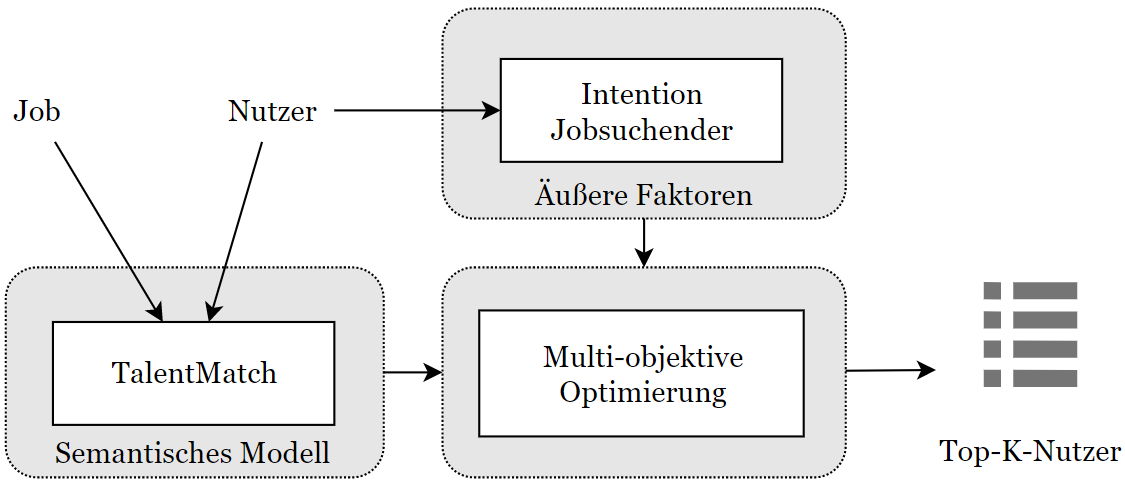
\includegraphics[width=0.9\textwidth]{gfx/talentMatch.png}
	\caption[Ansatz für die Integration äußerer Merkmale in semantische Modelle]{Ansatz für die Integration äußerer Merkmale in semantische Modelle\\
    (Eigene Darstellung in Anlehnung an \cite[S. 12]{rodriguez:inproceedings})}
	\label{fig:relatedwork:abb1}
\end{figure}

Im Detail stellen die Autoren eine Erweiterung des bestehenden \textit{TalentMatch}-Systems des sozialen Netzwerks LinkedIn vor, welche neben des semantischen Matches \cite[S. 2]{jannach:2:inproceedings} zwischen einer Person und einem Job (Objective 1) zusätzlich die Offenheit einer Person für einen Jobwechsel (Objective 2) in die Empfehlungserstellung (Ranking) miteinbezieht.
Dabei gehen die Autoren davon aus, dass die beiden Ziele möglicherweise miteinander konkurrieren, d.h. dass eine Person, die am besten auf eine Jobbeschreibung zutrifft, möglicherweise nicht offen für eine neue Stelle ist.
\textcite[S. 12]{rodriguez:inproceedings} untersuchen in ihrer Arbeit, ob die Berücksichtigung der Neigung von Personen für offene Jobpositionen den Nutzen der Nutzer des Systems dennoch positiv beeinflusst.
Den Nutzen operationalisieren die Autoren als das Engagement zwischen Jobsuchenden und Anbietern von Jobpositionen \cite[S. 14]{rodriguez:inproceedings}, welche diese über Menge aktiver, passiver und inaktiver Nutzer in dem System messen.
Die Integration der Berücksichtigung in das semantische Modell führen \textcite[S. 15]{rodriguez:inproceedings} systematisch über ein Re-Ranking durch.
Dies realisieren die Autoren über folgende Verlust-Funktion $L$ \cite[S. 13]{rodriguez:inproceedings}:
\begin{equation}\label{eq30}
    L(\alpha ,\beta) = -g(f(Y, X, [\alpha , \beta])) + \lambda \Delta (\pi (Y), \pi (f(Y,X,[\alpha ,\beta])))
\end{equation}
Nach \textcite[S. 15]{rodriguez:inproceedings} gibt Funktion $g$ die durchschnittliche Anzahl aktiver und passiver Nutzer in dem erweiterten System $f(Y, X, [\alpha , \beta])$ aus und $\Delta$ die Abweichung des Rankings $\pi (f(Y,X,[\alpha ,\beta]))$ des erweiterten Systems von dem Ranking $\pi (Y)$ des ursprünglichen semantischen Modells.
$\lambda$ stellt einen positiven Trade-Off-Parameter dar \cite[S. 13]{rodriguez:inproceedings}.
% \textcite[S. 13]{rodriguez:inproceedings} merken an, dass die Verlust-Funktion auch als Maximierungsproblem der Funktion $g$ dargestellt werden kann, welches $\Delta$ durch das Aufstellen einer Bedingung $c$ (d.h. $\Delta (\pi (Y), \pi (f(Y,X,[\alpha ,\beta]))) \leq c$) begrenzen kann.
Die Anpassung eines semantischen Matches $y$ realisieren \textcite[S. 15]{rodriguez:inproceedings} durch einen sogenannten "Boost", wobei zwischen einem Boost für aktive ($\alpha$) und passive ($\beta$) Nutzer unterschieden wird:
\begin{equation}\label{eq31}
    f(y,x,[\alpha ,\beta]) = y \times (\alpha^{1\{{x == \textnormal{active}\}}}) \times (\beta^{1\{{x == \textnormal{active}\}}})
\end{equation}
Hierbei ist $1\{x == \textnormal{active}\}$ gleich $1$, wenn die Bedingung innerhalb der geschweiften Klammer wahr ist und $0$ andernfalls.
Das Optimieren der Parameter $\alpha$ und $\beta$ führen \textcite[S. 15]{rodriguez:inproceedings} über eine Rastersuche durch.

\textcite[S. 15f.]{rodriguez:inproceedings} prüften ihren Ansatz anhand von 760 offenen Jobangeboten, von denen jedes zwischen 6 und 9000 mal in Empfehlungen auftauchte.
Dabei stellten die Autoren fest, dass eine signifikante Verbesserung des Nutzens mit einer akzeptablen und vorhersebaren Verschlechterung der semantischen Matches erreicht werden konnte \cite[S. 11]{rodriguez:inproceedings}.
% Dabei stellten die Autoren fest, dass bis zu einem gewissen Wert für Delta ein linearer Zusammenhang zwischen dem Zugewinn an durchschnittlich aktiven und passiven Nutzern und der Aufgabe von Übereinstimmung der Rankings besteht \cite[S. 16]{rodriguez:inproceedings}.
% Für bestimmte Kombinationen von $\alpha$ und $\beta$ konnte die Anzahl aktiver und passiver Nutzer in dem Top-K-Ranking durch Anwendung des erweiterten Modells verdoppelt werden, ohne massive Einbußen in den semantischen Matches einzufahren.
Kritisch betrachten \textcite[S. 16]{rodriguez:inproceedings} an ihrem Ansatz, dass für die Wirksamkeit eines Modells im praktischen Einsatz überprüft werden muss, ob die durchschnittliche Anzahl aktiver und passiver Nutzer tatsächlich repräsentativ für das Engagement von Nutzern in einem System ist.

\subsection{Multi-kriterielle Bewertungen in Empfehlungssystemen}
% Erfinder des aggregation Funktion approaches: file://wsl%24/Ubuntu/home/masc6/Projects/masterarbeit/literatur/New_Recommendation_Techniques_for_Multicriteria_Rating_Systems.pdf
% Arbeit von Jannach wie hier beschrieben mit SVM: S. 102, file://wsl%24/Ubuntu/home/masc6/Projects/masterarbeit/literatur/E-Commerce.pdf
% multi-kriteria: Aggregation function approach: file://wsl%24/Ubuntu/home/masc6/Projects/masterarbeit/literatur/Recommending%20Hotels%20based%20on%20Multidimesional%20Customer%20Ratings.pdf
% ansatz von Tang: zusammenfügen mehrere feature bewertungen, sowie durchschnittsbewertung und kommentare, file:///C:/Users/masc6/Downloads/tdladmin,+TangandMcCalla_JoDI_final.pdf
% Slope one algorithmus und adaptive genetic algorithm von Hassan, S. 327, file://wsl%24/Ubuntu/home/masc6/Projects/masterarbeit/literatur/Imrpoving%20Prediction%20accuracy%20of%20multi-criteria%20recommender.pdf
% Liu et al.: Cluster von Nutzern, welche wichtigkeit einzelner Attribute angeben, zusammenfassung siehe hier S. 4, file:///C:/Users/masc6/Downloads/79_HDIOUD.pdf
% CCSD method, siehe: file:///C:/Users/masc6/Downloads/79_HDIOUD.pdf
% Wenn viele features: liwei et al (zsfsg. siehe hier: file://wsl%24/Ubuntu/home/masc6/Projects/masterarbeit/literatur/A%20Multi-criteria%20Recommender%20System%20Incorporating%20Intensity%20of%20Preferences.pdf )

Darüber hinaus existieren einige Ansätze verwandter Domänen, die ebenfalls für die automatisierte Zuordnung von Personen für Jobpositionen relevant sind.
% Hier ggf. verwandte arbeiten in anderen domänen anführen. (z.B. Online Dating, Education)

% was gibt es also nicht? -> Reziprozität als gewichtetes Kriterium (Präferenz der empfohlenen Person zählt nicht genauso viel wie Präferenz des Nutzers, kann daher als gewichtetes Kriterium einer Aggregation Function betrachtet werden, welche über historische daten erlernt werden kann)
% Neue anwendungsbereiche von multi-kriteriellen EMpfehlungen in domänen wie online dating: zitat von S. 553, file://wsl%24/Ubuntu/home/masc6/Projects/masterarbeit/literatur/Towards%20the%20Next%20Generation%20of%20Multi-Criteria%20Recommender.pdf

% Zusätzlich: Darstellung negativer Präferenzen, siehe S. 288: https://link.springer.com/content/pdf/10.1007/978-3-642-22362-4.pdf?pdf=button
% -> RECON mit negativen Präferenzen

 \shorthandon{"}